\paragraph{}En este proceso, el usuario asesor puede crear,
consultar, modificar o borrar reuniones de la aplicación.

\paragraph{}La figura \ref{diagramaNivel4-GestionarReuniones}
muestra el nivel de abstracción 4: Gestionar reuniones.

  \begin{figure}[!ht]
    \begin{center}
      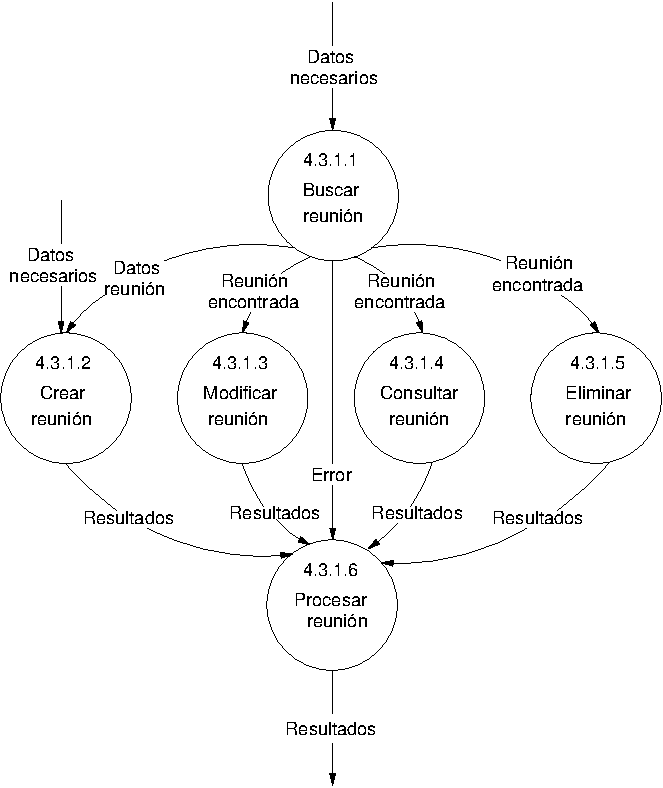
\includegraphics[]{08.Analisis_Funcional/8.2.DFDs/Niveles/Nivel4/Asesor/GestionarReuniones/Diagramas/nivel4-GestionarReuniones.pdf}
      \caption{Nivel de abstracción 4: Gestionar reuniones.}
      \label{diagramaNivel4-GestionarReuniones}
    \end{center}
  \end{figure}
